W oparciu o powy�sze wytyczne zaprojektowano schemat \ref{fig:PCBSCH} oraz p�ytk� PCB. Jako mikrokonroler zastosowano chip ATmega32 firmy ATmel, a konwerter napi�� dla RS-232 to popularny MAX232 w implementacji przetwornicy pojemno�ciowej. P�ytka zawiera kluczowanie zasilania sonar�w oraz w��czalny bypass dla sygna�u RC.

\begin{figure}[pt]
	\begin{center}
		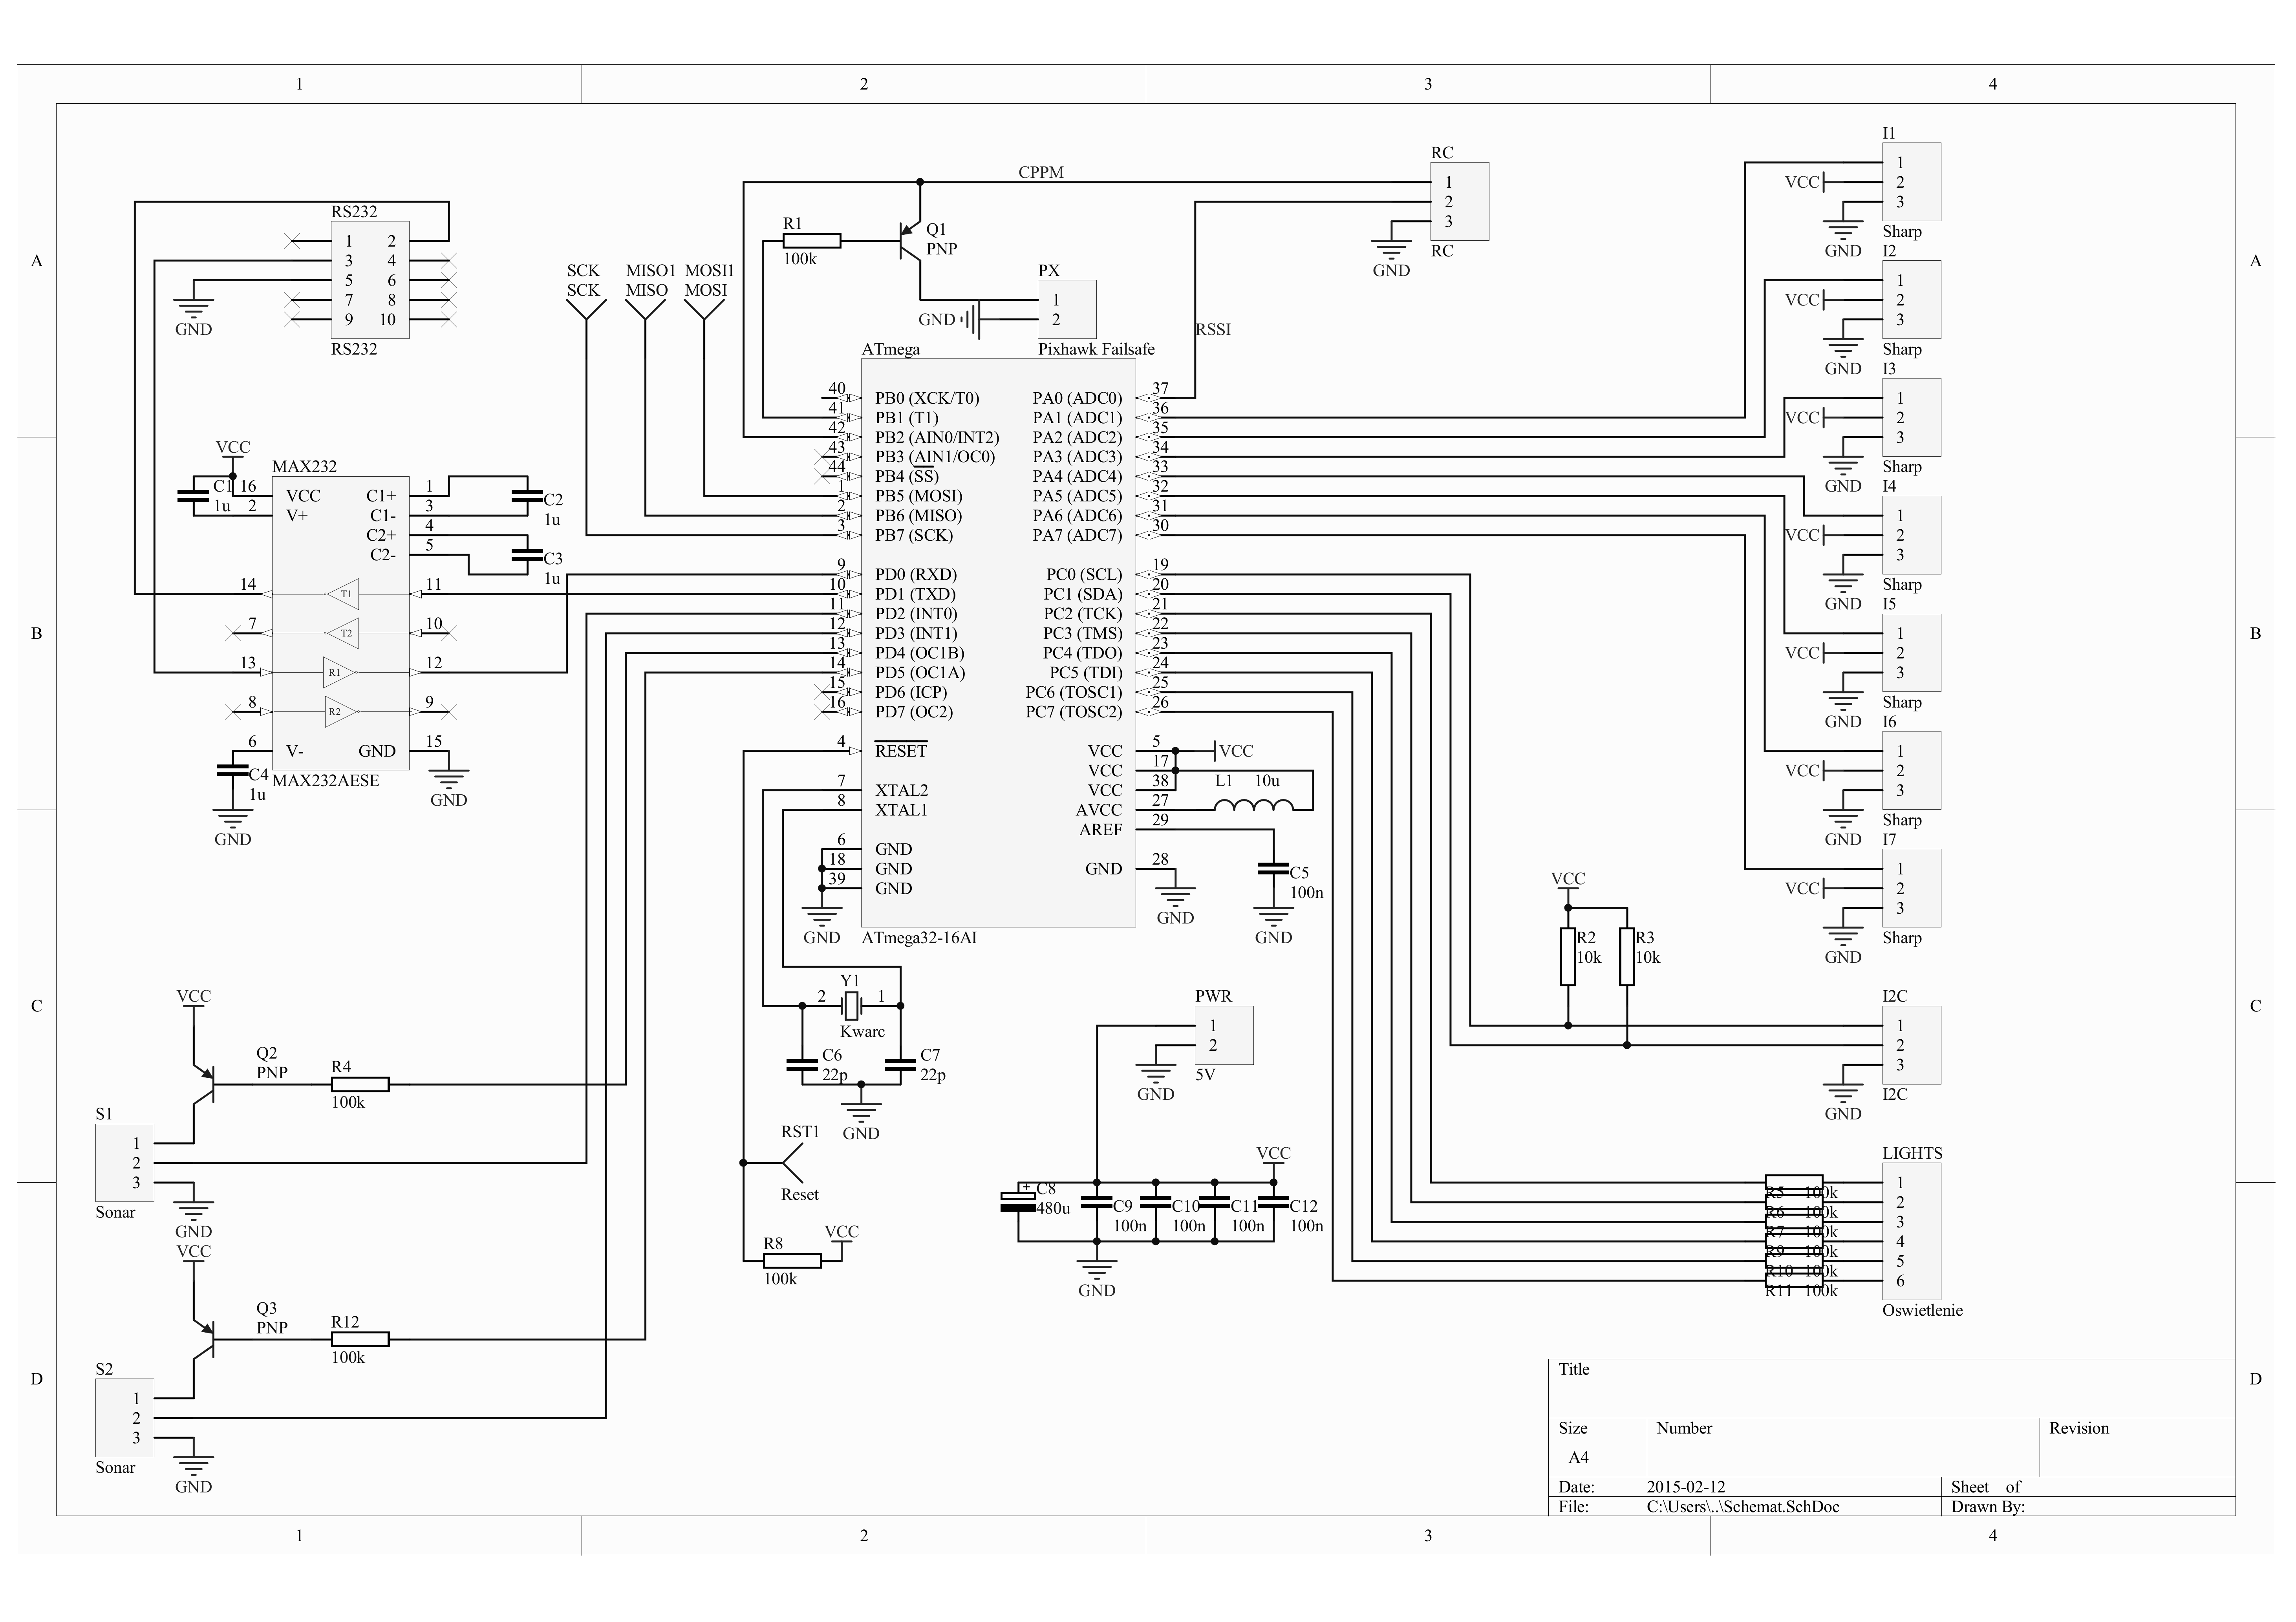
\includegraphics[width=0.85\textwidth]{grafika/schemat.png}
		\caption{Schemat p�ytki PCB}
		\label{fig:PCBSCH}
	\end{center}
\end{figure}

Opis z��cz znajduje si� na rys. \ref{fig:PCBZL}.

\begin{figure}[pt]
	\begin{center}
		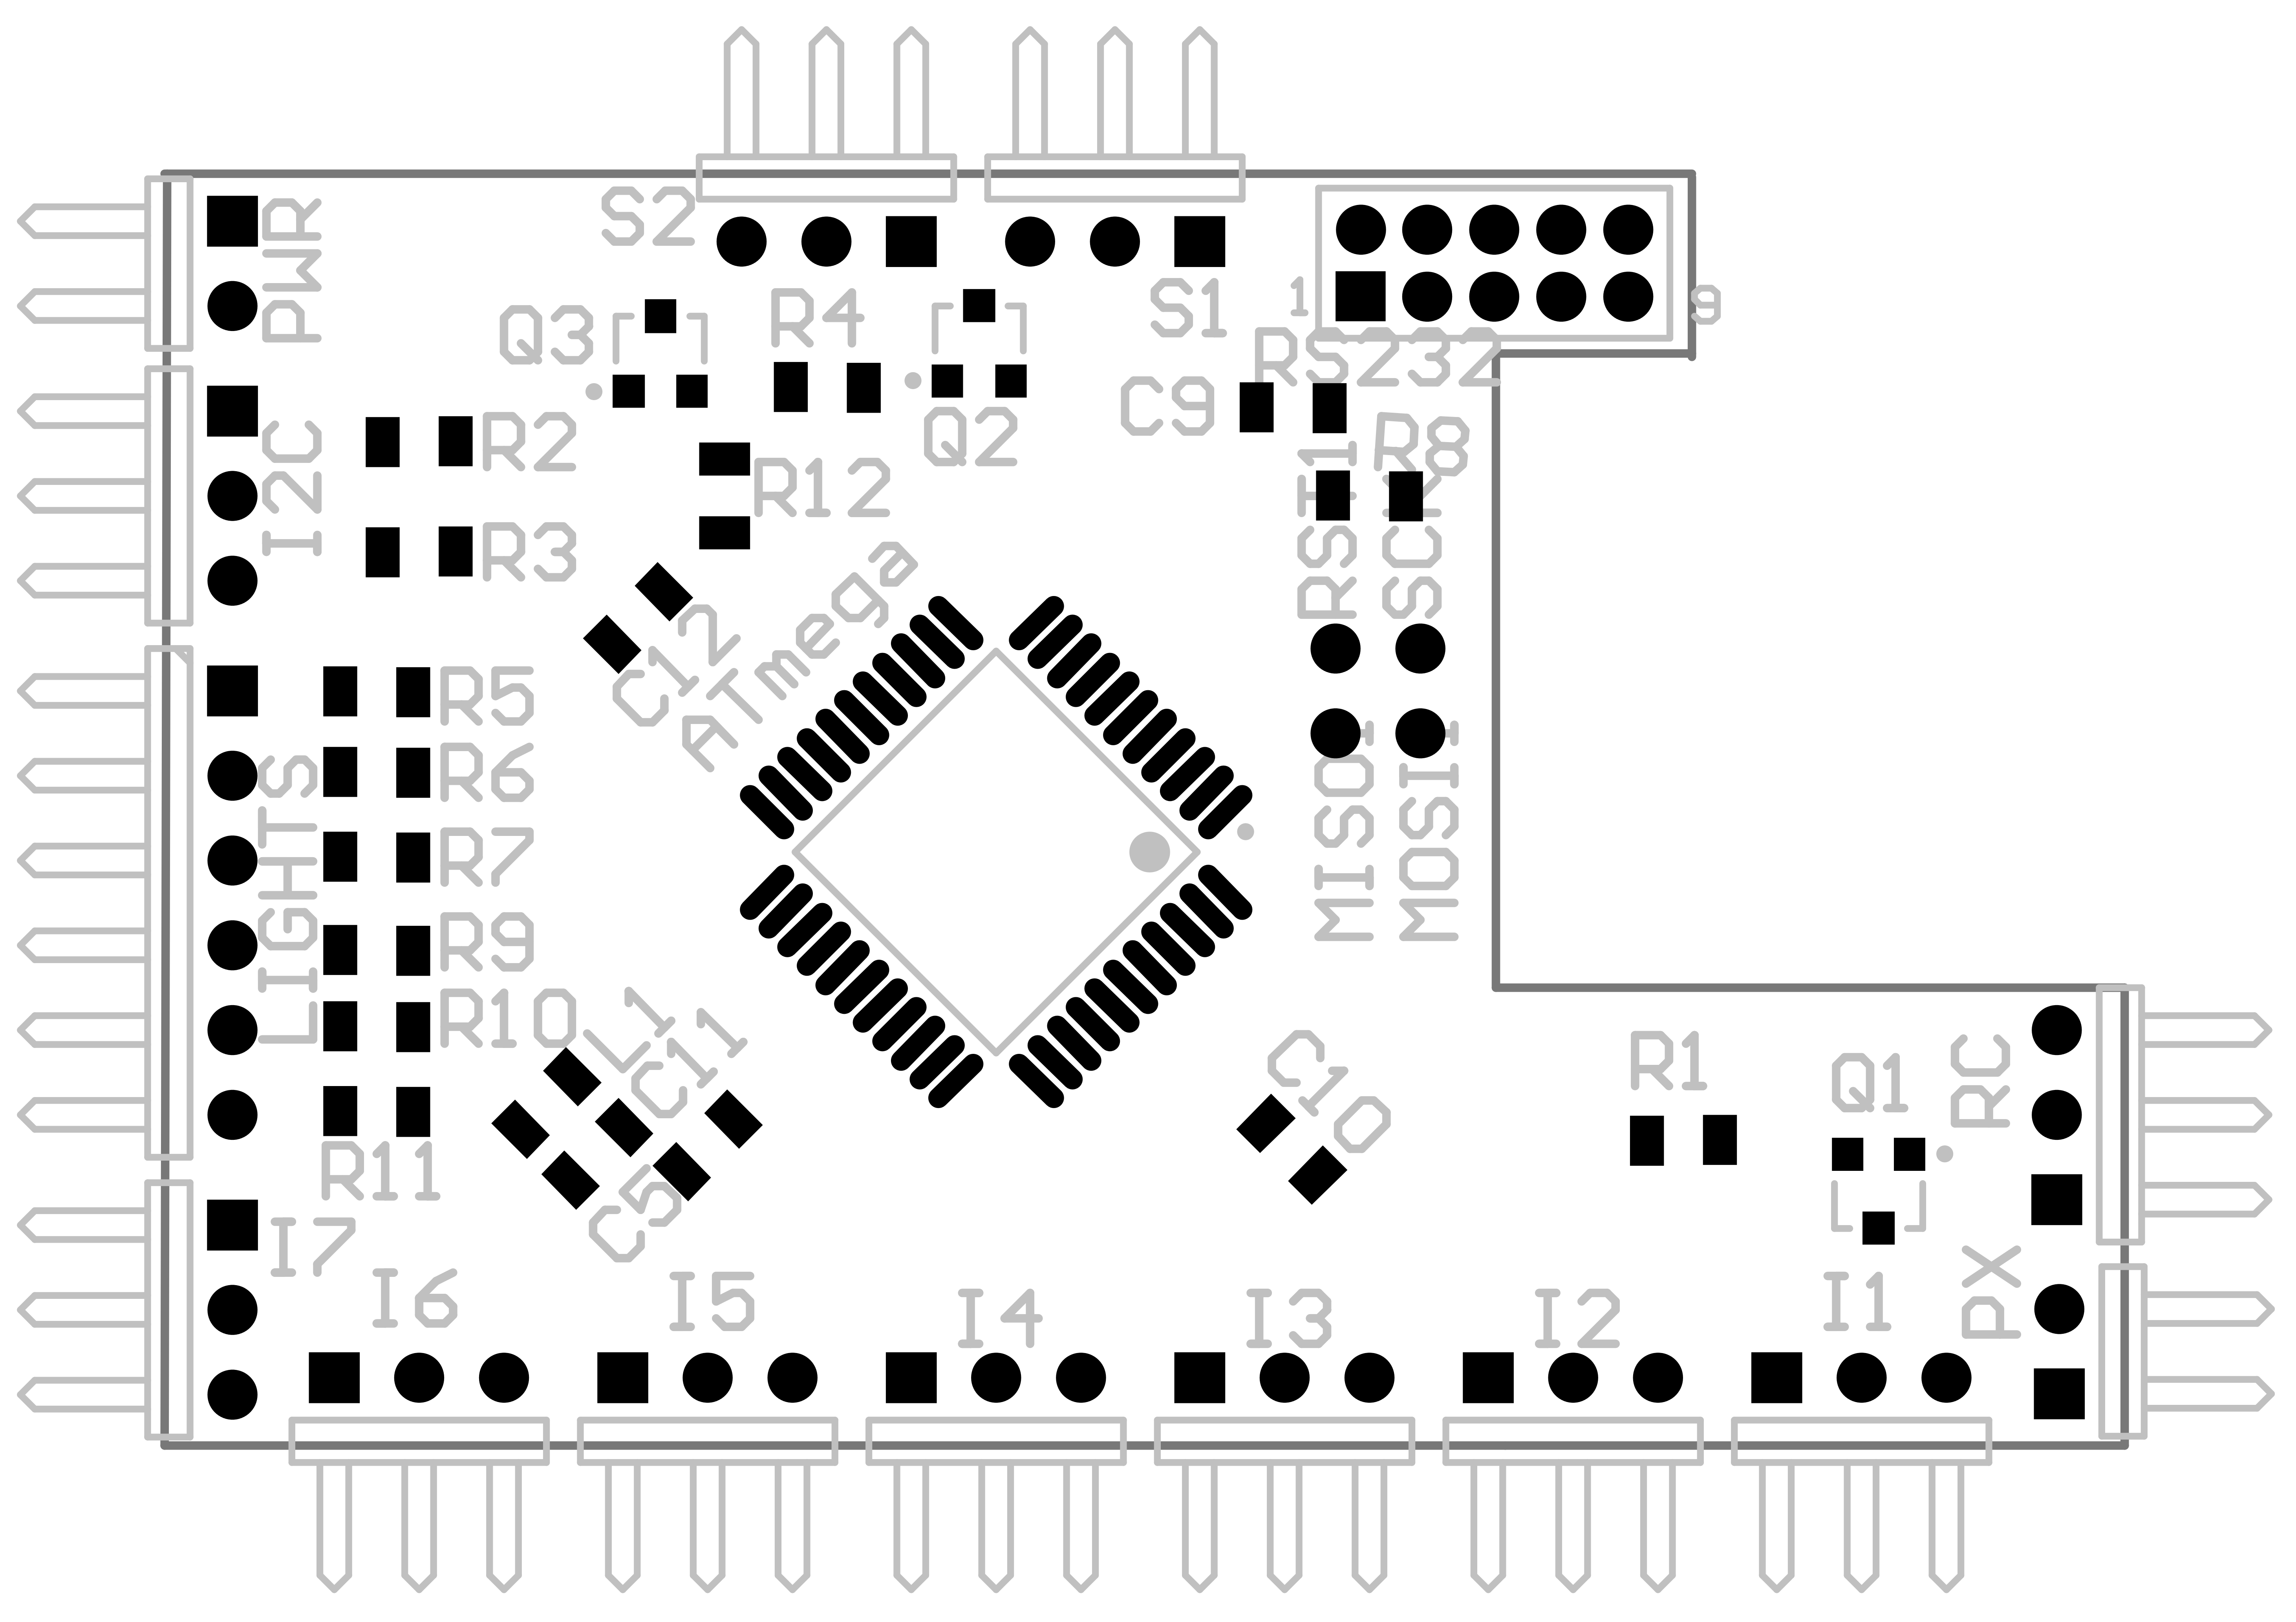
\includegraphics[width=0.85\textwidth]{grafika/zlacza.png}
		\caption{Schemat powierzchni g�rnej PCB. \\ Ix - wej�cia analogowe, \\ Sx - wej�cia PWM, \\ PX - z��cze RC dla \emph{Pixhawka}, \\ RC - Sygna� CPWM oraz RSSI \\ Kwadratowy pad jest pinem nr 1}
		\label{fig:PCBZL}
	\end{center}
\end{figure}


Na rysunku \ref{fig:interfejs} przedstawiono wykonany interfejs czujnik�w. Widoczne z��cza umo�liwiaj� pod��czenie zasilania, czujnik�w odleg�o�ci Sharp, stopnia mocy o�wietlenia, czy sygna�u z aparatury RC.


\begin{figure}[h!]
  \begin{center}
\subfigure[widok z g�ry]{
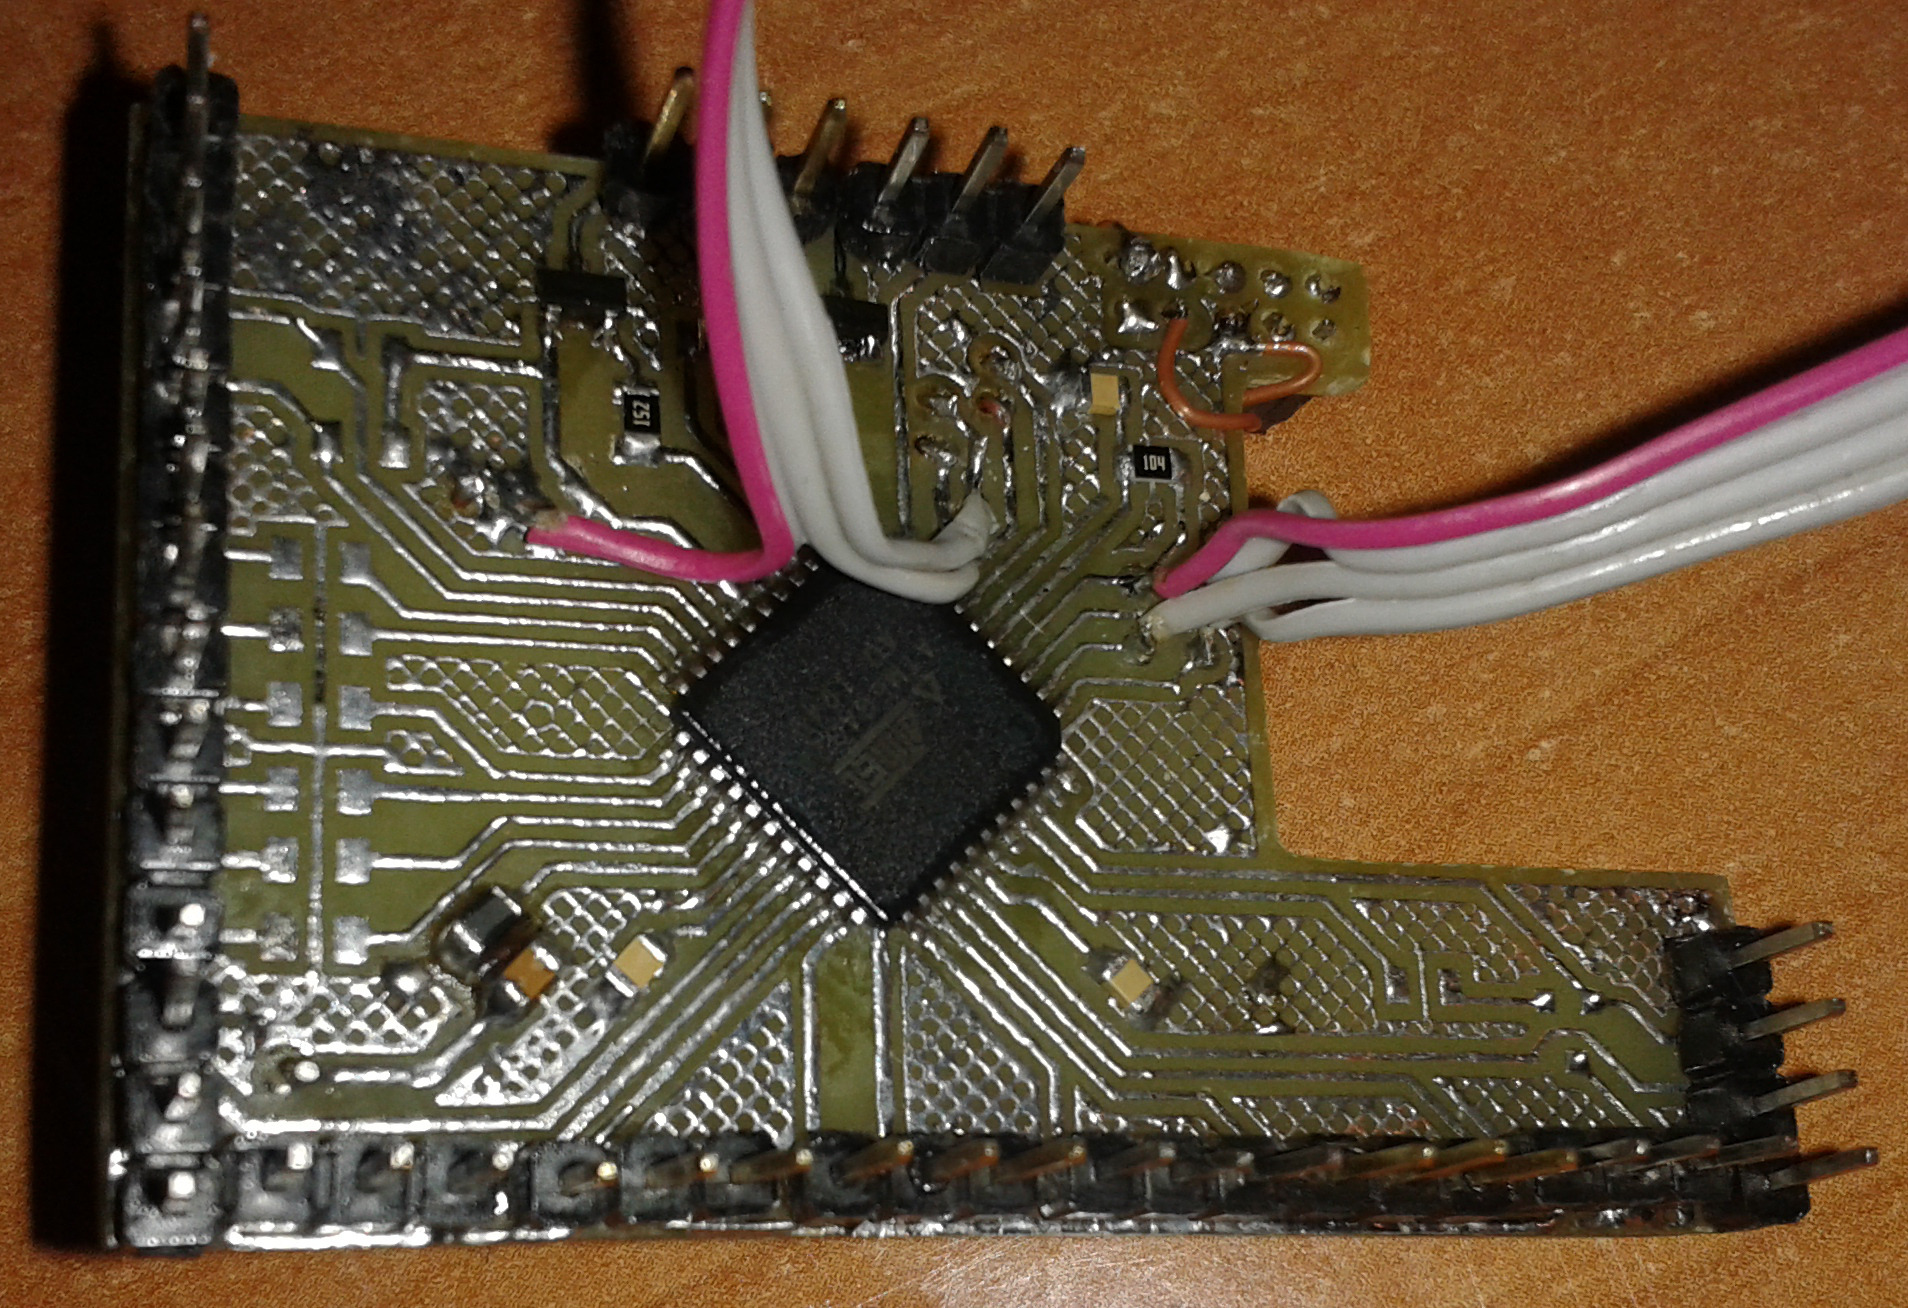
\includegraphics[angle=0, width=0.8\textwidth]{grafika/md_interfejs_gora.jpg}
\label{fig:interfejs_gora}
}
\subfigure[widok z do�u]{
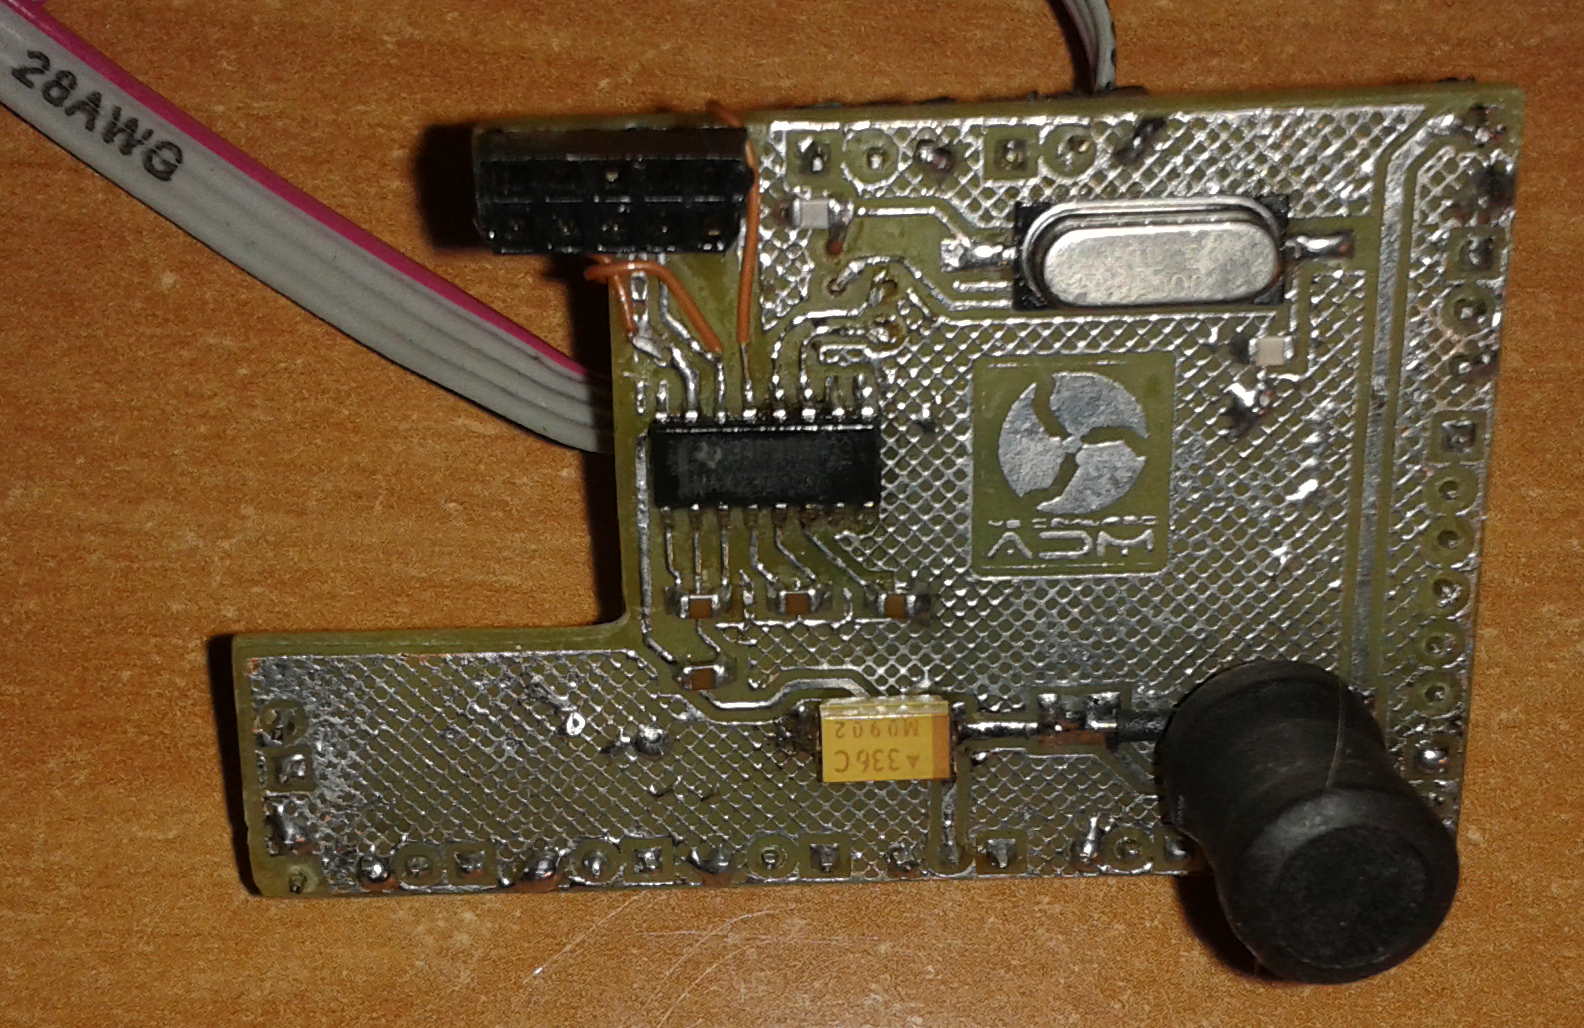
\includegraphics[angle=0, width=0.8\textwidth]{grafika/md_interfejs_dol.jpg}
\label{fig:interfejs_dol}
}
    \caption{Przedstawienie wykonanego interfejsu }
    \label{fig:interfejs}
  \end{center}
\end{figure}